% \chapter{Indicators overview}

\chapter{Supporting Documents}
\label{cha:attachment_overleaf_comparison}

\section{Overview of Indicators}
Figure \ref{fig:A1_attach_indicators_overview} provides an overview of the indicators defined in Chapter 3. In the figure, the indicators are accompanied by their dimensions, metrics, and results assignment criteria.

\section{Comparison between Overleaf versions}
Figure \ref{fig:A2_attach_overleaf_overview} presents a detailed comparison table of the different versions of Overleaf. The table includes features, integrations, and administration capabilities. Additionally, it provides the minimum installation requirements and a categorized list of sub-processors. For completeness, the pricing of the various plans is also included.

\newpage

% DIGITALE SENZA NUMERO
% 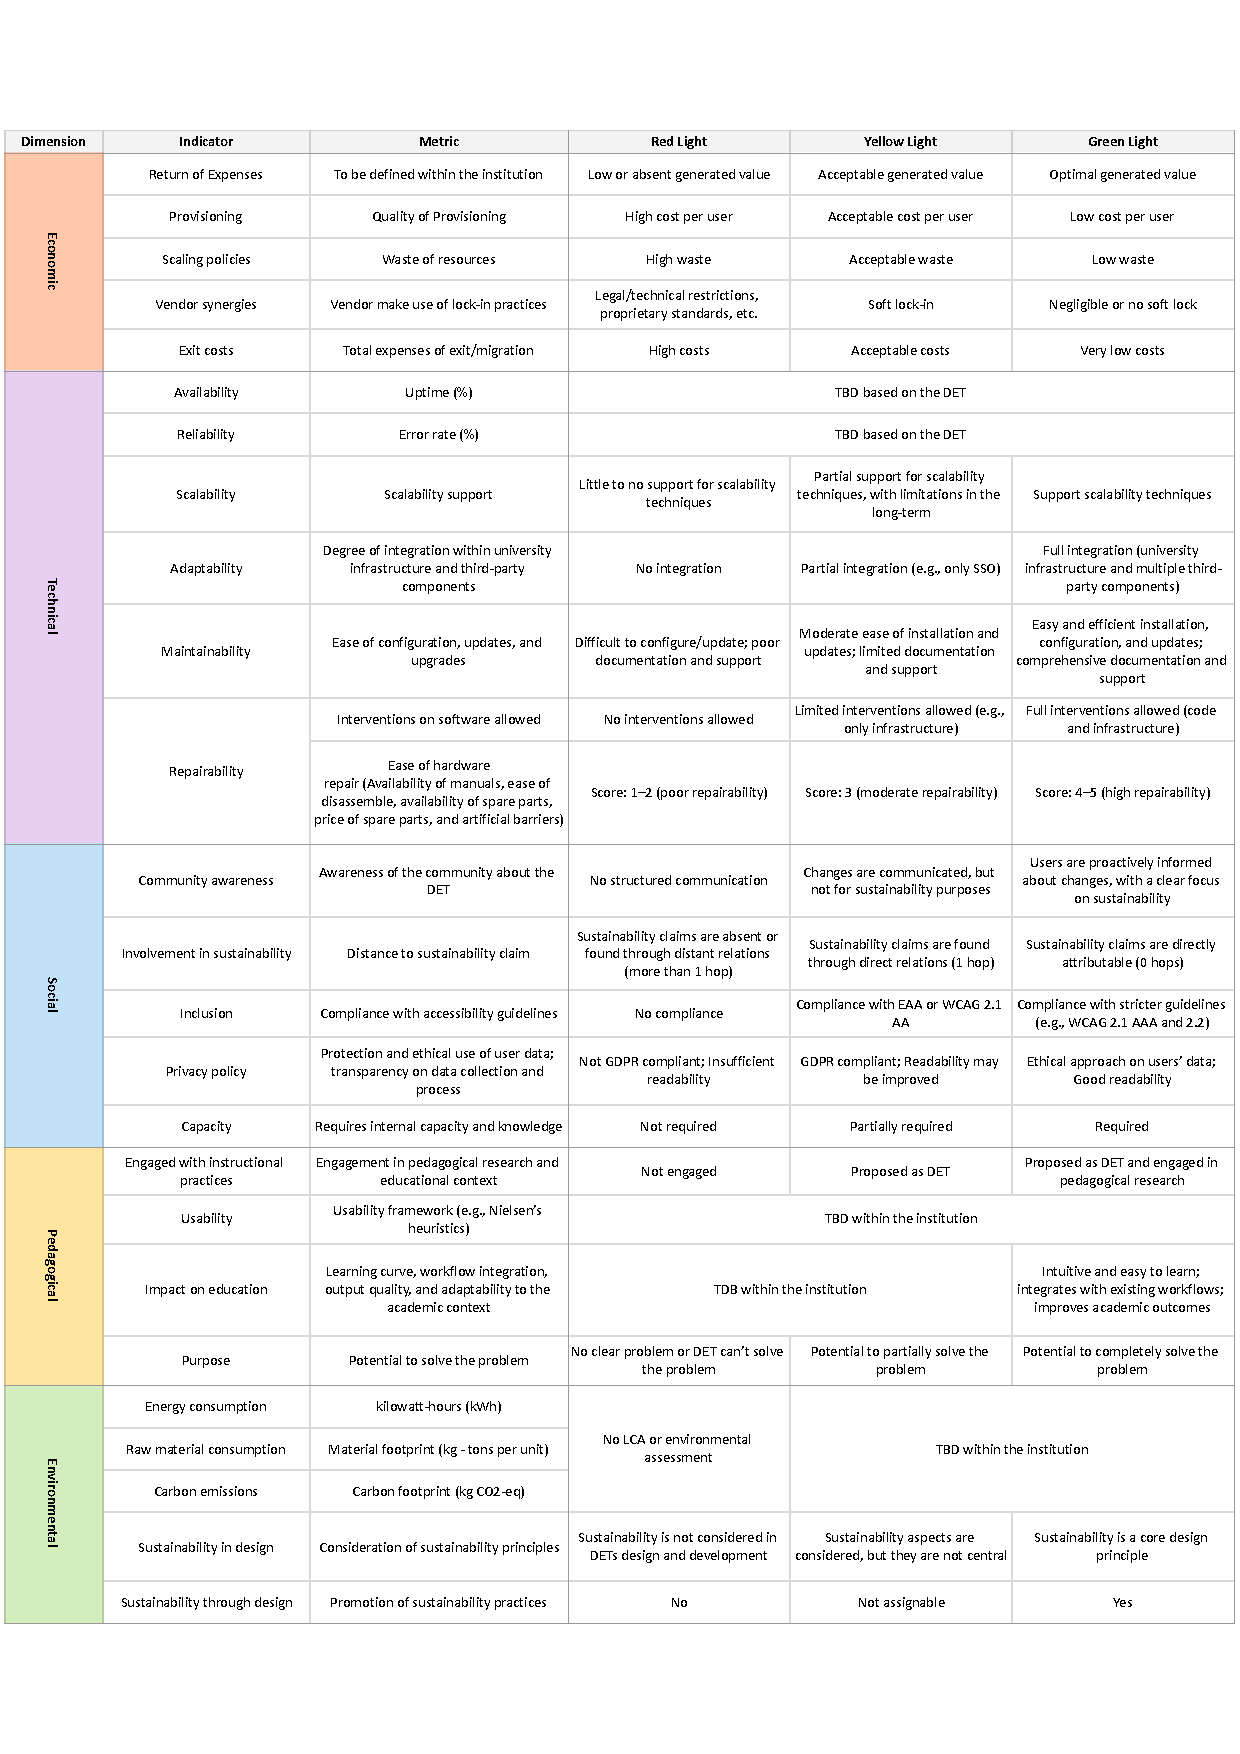
\includepdf[pages=1, fitpaper=true]{attachments/indicators_overview.pdf}
% 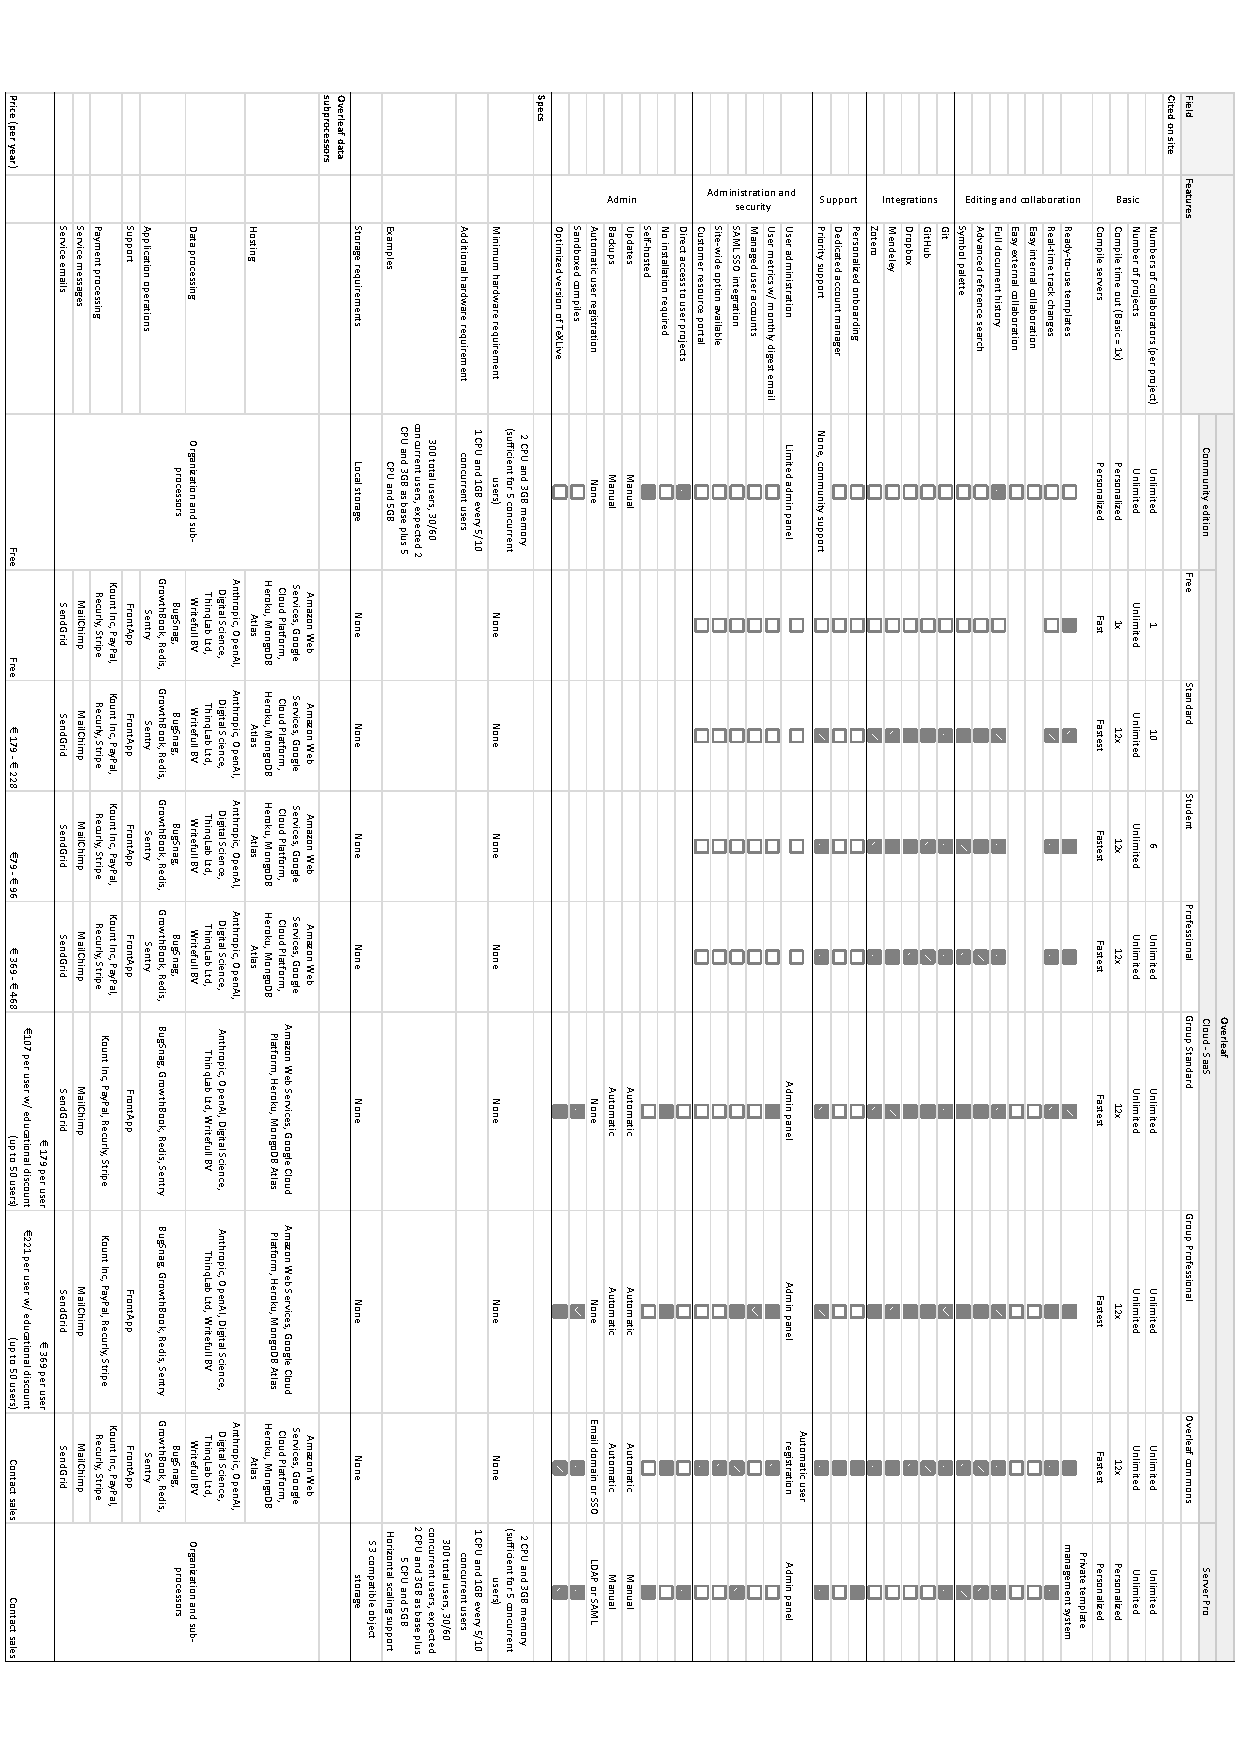
\includepdf[pages=1, fitpaper=true]{attachments/overleaf_overview.pdf}

% DIGITALE CON NUMERO
% \begin{figure}[ht]
%     \centering
%     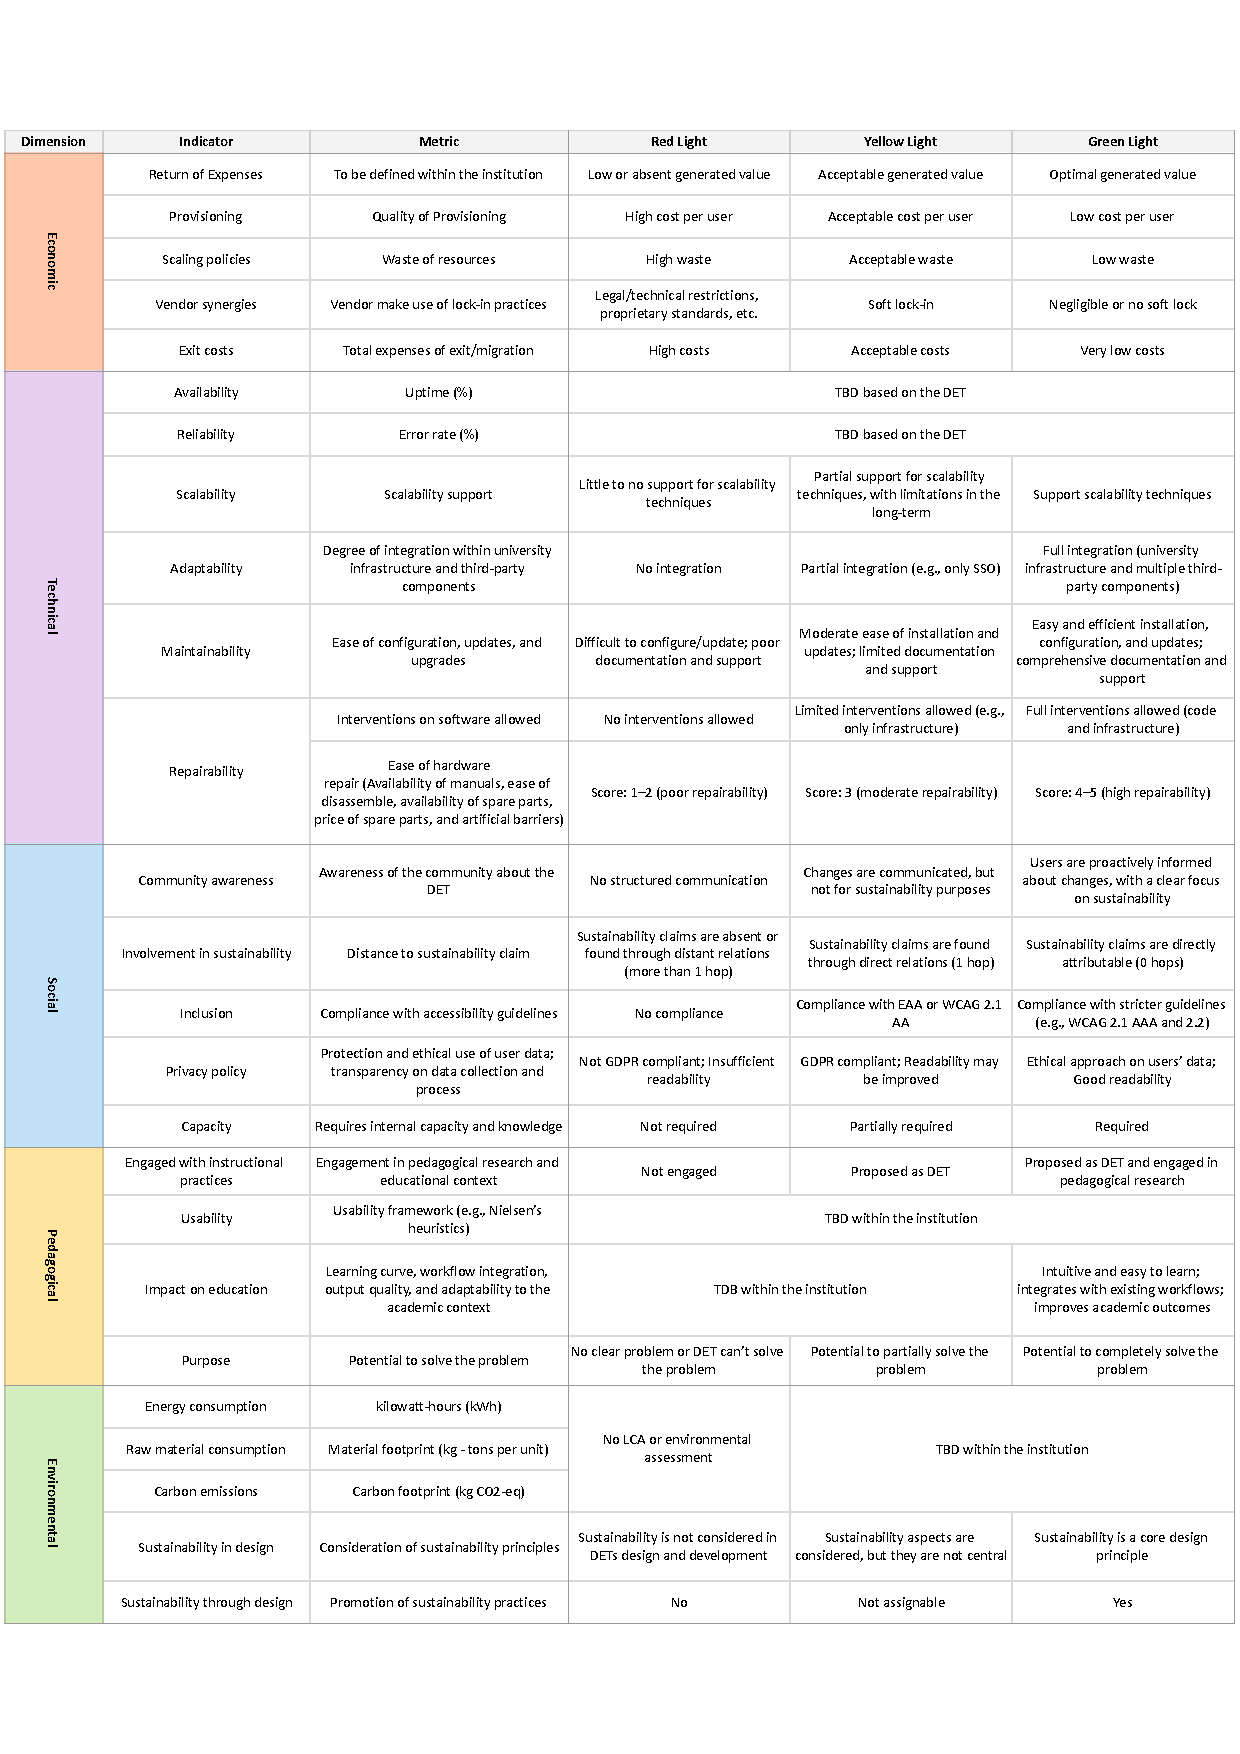
\includepdf[pages=1, scale=0.8]{attachments/indicators_overview.pdf}
%     \caption{Overview of indicators}
% \end{figure}

% \begin{figure}[ht]
%     \centering
%     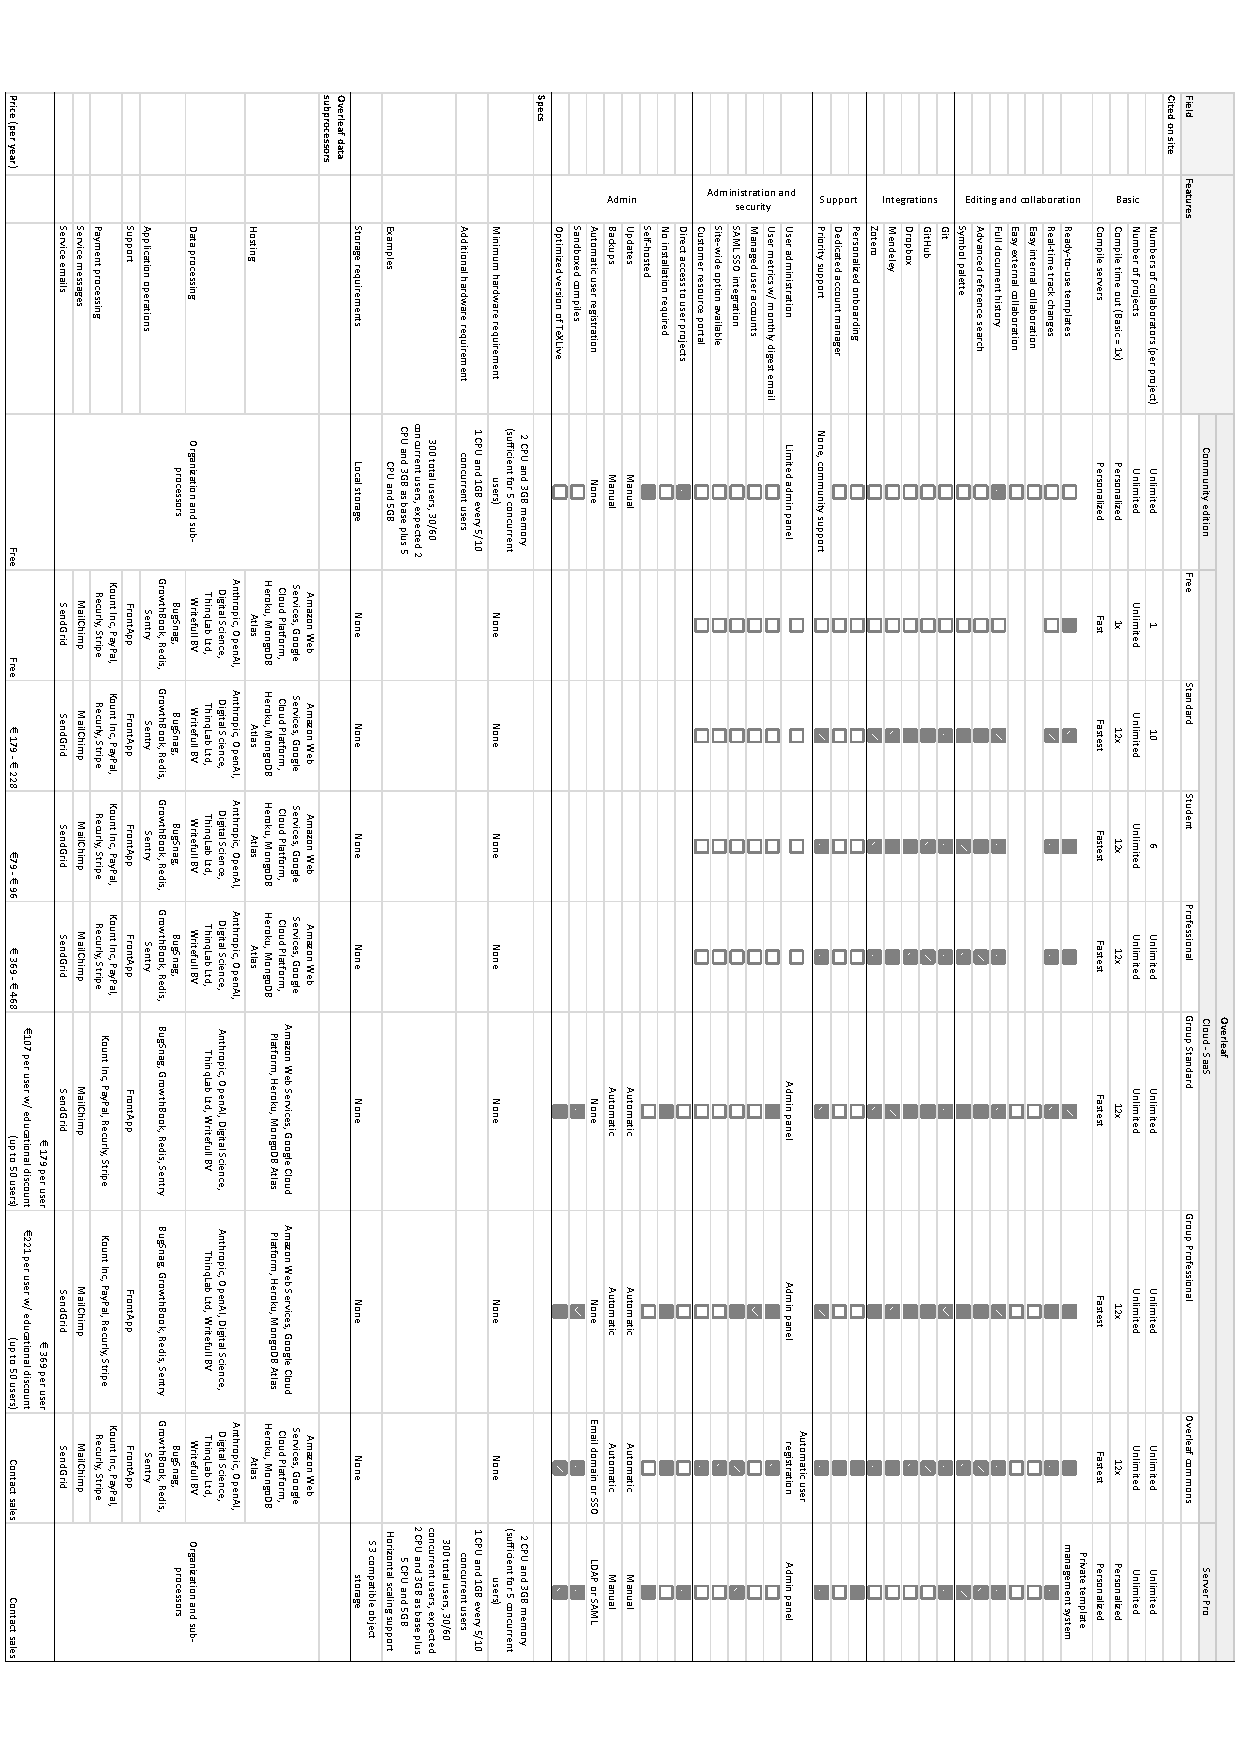
\includepdf[pages=1, scale=0.8]{attachments/overleaf_overview.pdf}
%     \caption{Comparison between Overleaf versions}
% \end{figure}

% STAMPA
\begin{figure}[ht]
    \centering
    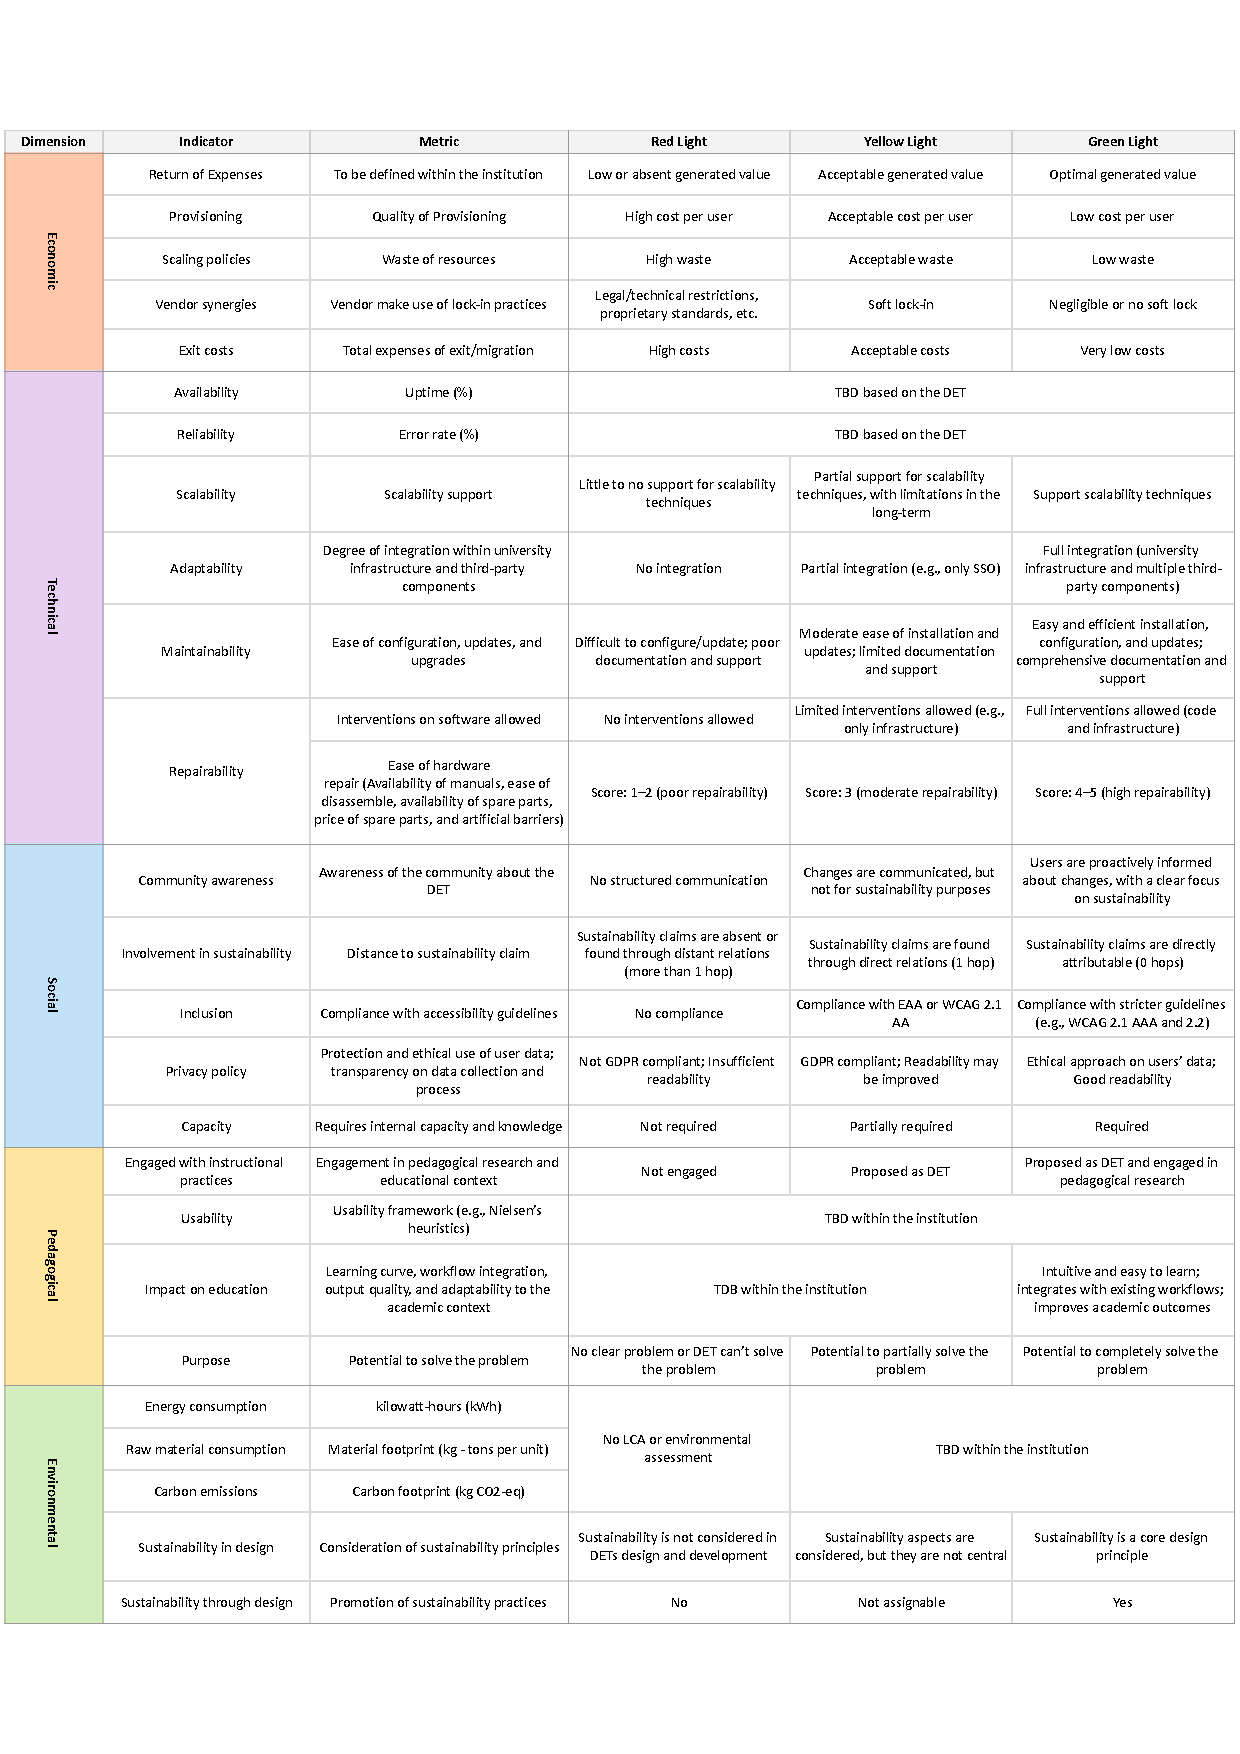
\includegraphics[width=1\linewidth]{attachments/indicators_overview.pdf}
    \caption{Overview of indicators}
    \label{fig:A1_attach_indicators_overview}
\end{figure}

\begin{figure}[ht]
    \centering
    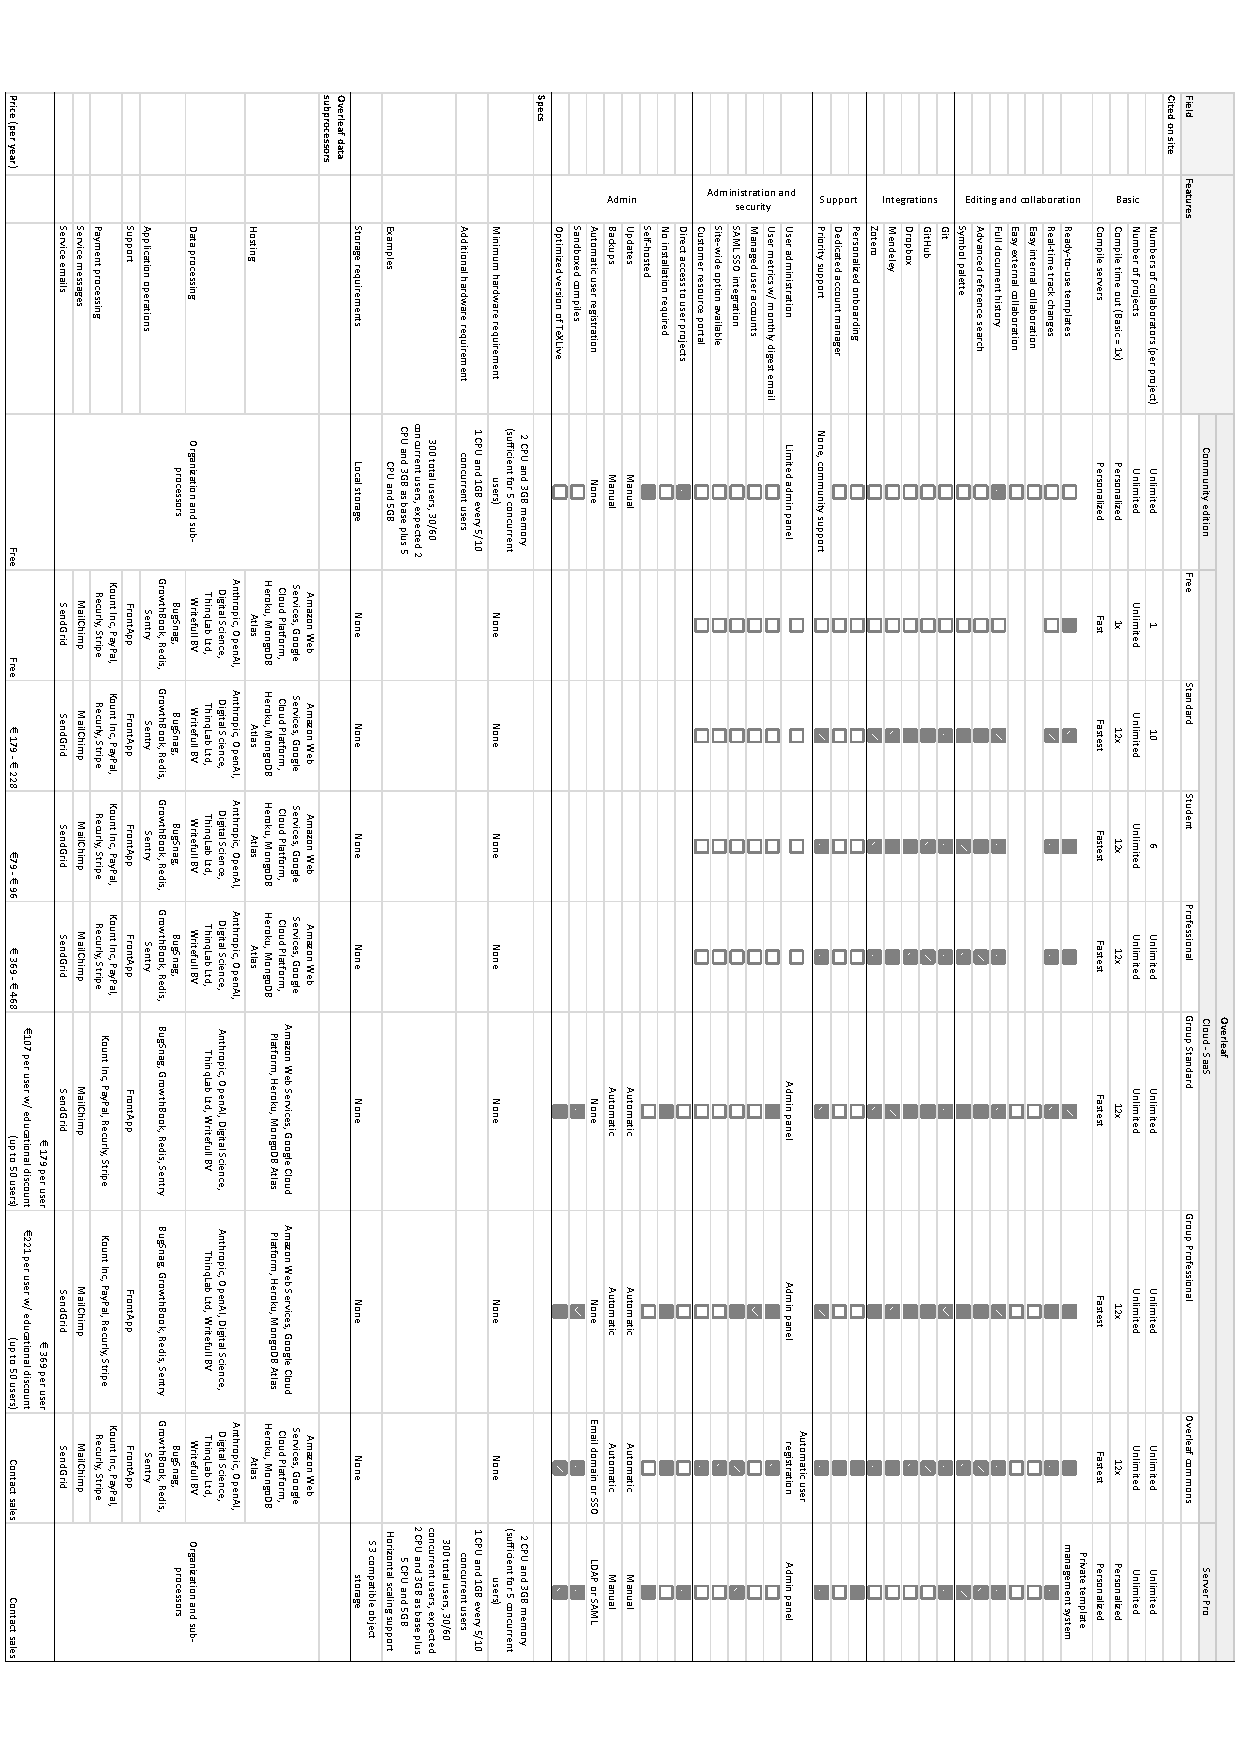
\includegraphics[width=1\linewidth]{attachments/overleaf_overview.pdf}
    \caption{Comparison between Overleaf versions}
    \label{fig:A2_attach_overleaf_overview}
\end{figure}

\newpage




